%% This template was written by Steven Miller and is available here: https://github.com/svmiller/svm-r-markdown-templates/blob/master/svm-latex-ms.tex %%

\documentclass[11pt,]{article}
\usepackage[left=1in,top=1in,right=1in,bottom=1in]{geometry}
\newcommand*{\authorfont}{\fontfamily{phv}\selectfont}
\usepackage[]{mathpazo}


  \usepackage[T1]{fontenc}
  \usepackage[utf8]{inputenc}



\usepackage{abstract}
\renewcommand{\abstractname}{}    % clear the title
\renewcommand{\absnamepos}{empty} % originally center

\renewenvironment{abstract}
 {{%
    \setlength{\leftmargin}{0mm}
    \setlength{\rightmargin}{\leftmargin}%
  }%
  \relax}
 {\endlist}

\makeatletter
\def\@maketitle{%
  \newpage
%  \null
%  \vskip 2em%
%  \begin{center}%
  \let \footnote \thanks
    {\fontsize{18}{20}\selectfont\raggedright  \setlength{\parindent}{0pt} \@title \par}%
}
%\fi
\makeatother




\setcounter{secnumdepth}{0}


\usepackage{graphicx}
% We will generate all images so they have a width \maxwidth. This means
% that they will get their normal width if they fit onto the page, but
% are scaled down if they would overflow the margins.
\makeatletter
\def\maxwidth{\ifdim\Gin@nat@width>\linewidth\linewidth
\else\Gin@nat@width\fi}
\makeatother
\let\Oldincludegraphics\includegraphics
\renewcommand{\includegraphics}[1]{\Oldincludegraphics[width=\maxwidth]{#1}}

\title{Frequency and Intensity: Cyanobacterial Blooms in Nebraska Freshwater Bodies  }



\author{\Large Victoria Wickham\vspace{0.05in} \newline\normalsize\emph{Batchelor of Science in Water Science from the College of Agricultural
Sciences and Natural Resources, University of Nebraska-Lincoln}   \and \Large Dr.~Megan L. Larsen\vspace{0.05in} \newline\normalsize\emph{Water Sciences Laboratory, University of Nebraska-Lincoln}  }


\date{}

\usepackage{titlesec}

\titleformat*{\section}{\normalsize\bfseries}
\titleformat*{\subsection}{\normalsize\itshape}
\titleformat*{\subsubsection}{\normalsize\itshape}
\titleformat*{\paragraph}{\normalsize\itshape}
\titleformat*{\subparagraph}{\normalsize\itshape}


\usepackage{natbib}
\bibliographystyle{apsr}
\usepackage[strings]{underscore} % protect underscores in most circumstances



\newtheorem{hypothesis}{Hypothesis}
\usepackage{setspace}

\makeatletter
\@ifpackageloaded{hyperref}{}{%
\ifxetex
  \PassOptionsToPackage{hyphens}{url}\usepackage[setpagesize=false, % page size defined by xetex
              unicode=false, % unicode breaks when used with xetex
              xetex]{hyperref}
\else
  \PassOptionsToPackage{hyphens}{url}\usepackage[unicode=true]{hyperref}
\fi
}

\@ifpackageloaded{color}{
    \PassOptionsToPackage{usenames,dvipsnames}{color}
}{%
    \usepackage[usenames,dvipsnames]{color}
}
\makeatother
\hypersetup{breaklinks=true,
            bookmarks=true,
            pdfauthor={Victoria Wickham (Batchelor of Science in Water Science from the College of Agricultural
Sciences and Natural Resources, University of Nebraska-Lincoln) and Dr.~Megan L. Larsen (Water Sciences Laboratory, University of Nebraska-Lincoln)},
             pdfkeywords = {harmful algal blooms, frequency, intensity, Nebraska lakes},  
            pdftitle={Frequency and Intensity: Cyanobacterial Blooms in Nebraska Freshwater Bodies},
            colorlinks=true,
            citecolor=blue,
            urlcolor=blue,
            linkcolor=magenta,
            pdfborder={0 0 0}}
\urlstyle{same}  % don't use monospace font for urls



% add tightlist ----------
\providecommand{\tightlist}{%
\setlength{\itemsep}{0pt}\setlength{\parskip}{0pt}}

\begin{document}
	
% \pagenumbering{arabic}% resets `page` counter to 1 
%
% \maketitle

{% \usefont{T1}{pnc}{m}{n}
\setlength{\parindent}{0pt}
\thispagestyle{plain}
{\fontsize{18}{20}\selectfont\raggedright 
\maketitle  % title \par  

}

{
   \vskip 13.5pt\relax \normalsize\fontsize{11}{12} 
\textbf{\authorfont Victoria Wickham} \hskip 15pt \emph{\small Batchelor of Science in Water Science from the College of Agricultural
Sciences and Natural Resources, University of Nebraska-Lincoln}   \par \textbf{\authorfont Dr.~Megan L. Larsen} \hskip 15pt \emph{\small Water Sciences Laboratory, University of Nebraska-Lincoln}   

}

}







\begin{abstract}

    \hbox{\vrule height .2pt width 39.14pc}

    \vskip 8.5pt % \small 

\noindent Some really good stuff here with 1-2 sentences from the INTRO, RESULTS,
and CONCLUSIONS. This section should be no longer than 300 words.


\vskip 8.5pt \noindent \emph{Keywords}: harmful algal blooms, frequency, intensity, Nebraska lakes \par

    \hbox{\vrule height .2pt width 39.14pc}



\end{abstract}


\vskip 6.5pt

\noindent   \clearpage
\tableofcontents  \newpage
\listoftables  \newpage
\listoffigures  \newpage

\section{Introduction}\label{introduction}

Cyanobacteria (also known as blue-green algae) are ancient
photosynthetic microbes found across diverse habitats. These organisms
are an important part of the aquatic food chain, but some species
produce potent compounds, known as cyanotoxins, that pose a risk to
humans, fish, and invertebrates. Events where the amount of
cyanobacteria, and their subsequent cyanotoxins, are so great that they
pose a threat to humans, or cause ecological or economic harm, is called
a harmful algal bloom (HAB). Cyanobacterial toxin poisonings are a large
component of the concerns surrounding harmful algal blooms, and have
been the major driver behind the increase in attention being put on them
in the last decade.

Cyanobacterial HABs can cause harm in many different ways: By causing
sickness and death in humans, animals, fish, and invertebrates, by
causing harm to an ecosystem by decreasing the quality and ecosystem
health of a water body, and by causing economic harm by impairing water
bodies to such a degree that they cannot be used for drinking,
irrigation, fishing, recreation, or aquaculture.

Harm to living organisms comes from the side-effects of ingesting
cyanotoxins. Cyanobacterial toxin poisonings (CTP) in humans are a rare
occurrence, primarily because humans avoid water bodies with high toxic
cell concentrations. Cyanotoxins can be present in finished water
supplies, however, as the removal of cyanotoxins in this way is not
always efficient (Paerl and Otten 2012). The implication of this is that
they can be a potential danger to both humans and animals (Blaha,
Babica, and Marsalek, 2009). When oral poisonings have occurred, such as
through improperly treated drinking water supplies, reported symptoms
include abdominal pain, nausea, vomiting, diarrhea, sore throat, dry
cough, headache, blistering of the mouth, atypical pneumonia, and
elevated liver enzymes (Chorus and Bartram, 1999). In most of these
cases, as with most instances of human poisonings due to cyanotoxins,
the levels of toxin have not been identified. In other cases, human
poisonings have been suspected but were not confirmed due to a lack of
information (Carmichael et al, 2001). The most common exposure route for
humans is through recreational waters, consumption of drinking water,
and algal health food tablets. There have been no known fatalities
through these oral and dermal routes. The only cause of human fatalities
due to cyanotoxins was through intravenous exposure from a dialysis
clinic in Caruaru, Brazil in 1996. Symptoms of the exposure, now
referred to as Caruaru Syndrome, included painful enlargement of the
liver, jaundice, and an increased tendency to suffer from metrorrhagia,
nose bleeds, and hemorrhagic spots. (Carmichael et al, 2001).

The presence of cyanobacterial HABs can negatively impact the health of
a water body and its ecosystem. The blooms themselves alter the physical
and chemical makeup of the surrounding water. They do this by
deoxygenating the hypolimnion, which in turn releases nutrients from the
sediment, releasing hydrogen sulfide and methane, and by producing
cyanotoxins. These changes can cause a reduction or even an elimination
of benthic flora and fauna, as well as a decrease in the amount of
desirable plant species, including algae (Paerl, 1988). In fact,
cyanobacterial blooms may drive cascading trophic impacts due to their
toxicity and palatability which may then drive food webs in affected
lakes to switch from planktonic to benthic or detrital in response
(Paerl, 1988). Cyanobacterial blooms also increase turbidity in the
water body, which decreases light penetration to lower levels. This,
naturally, decreases the ability for macrophytes and benthic microalgae
to establish, which ultimately affects underwater habitat for other
species (Jeppesen et al, 2007; Scheffer et al, 1997; Scheffer 2004).

Economic harm from cyanobacterial HABs comes from the impairment of
water bodies. These water bodies can be affected to such a degree that
they can no longer be used for their intended purposes, such as
recreation, drinking, irrigation, fishing, and aquaculture. Estimating
the cost of ecosystem services or damage is always incredibly difficult,
and relies on making certain assumptions, which may or may not be true
in real-world application. Regardless, cost estimations have been made.
Hoagland et al. estimated that harmful algal blooms cost the United
States approximately 46 million dollars a year. This estimate takes
costs associated with shellfish poisonings, ciguatera fish poisonings,
commercial fishery damage, untapped fishery resources, losses associated
with recreation and tourism, and the costs of monitoring and management
into account (Hoagland et al, 2002). Anderson et al. had a much higher
estimate at 449 million dollars per year. This estimate summed the costs
associated with public health, commercial fisheries, recreation and
tourism, and monitoring and management (Anderson et al, 2000). Both
studies found that the highest costs were associated with public health.
This highlights the need to understand bloom mechanisms and trends.

Throughout the literature, there has thought to have been an increase in
the number, distribution, and intensity of harmful algal blooms. The
evidence presented above illustrates why it is very important to
quantify if this is true or not, and this question has been approached
from several different angles in a number of papers.

The original paper that set this idea forward mainly looked at the
global distribution of shellfish poisonings (Hallegraff, 1993). The
interesting thing to note here is that this paper doesn't really go into
the intensity or frequency of these blooms themselves, but simply looks
at the instances of reported shellfish poisonings that are caused by
cyanotoxins. The author himself acknowledges that the apparent global
increase that he sets forward may not be a real increase, but may simply
be the result of increased detection and awareness. He is not the only
author to frame an increase in cyanobacterial blooms in this way. Chung
et al. argues that there is an increase in HABs worldwide, and that this
is reflected by the fact that there has also been an increasing number
of reports and studies on cyanobacterial blooms in the last decade
(Cheung et al, 2013). Again, these authors acknowledge that this trend
could be due to increased detection and awareness. Other papers on the
subject use the phrase ``apparent increase'', but few actually tackle
the question head-on.

Another paper by Loftin et al, looked at the concentration and
distribution of cyanotoxins across the United States using data from the
EPA National Lakes Assessment 2007 (Loftin et al, 2016). Although
informative, this paper is simply a nationwide snapshot of distribution
and concentration, and does not address increasing frequency over time.
Taranu et al. analyzed paleolimnological pigment sediment core records
in order to determine how cyanotoxins have increased since the 1800s.
They found that cyanobacteria have increased significantly since the
1800s, have increased disproportionately relative to other
phytoplankton, and have increased more rapidly since 1945 (Taranu et al,
2015). These findings are a step in the right direction, but the amount
of actual toxin could not be measured using this method. Therefore,
conclusions about intensity could not be made. A study comparing the
findings presented here with actual toxin amounts in grab samples from
the past decade, could be a valuable addition to these findings.

Reasons given for this apparent increase in frequency and intensity are
eutrophication due to increased nutrient loading, increasing water
temperatures due to climate change, increased vigilance, advances in
monitoring efforts and analytical techniques, and anthropogenic
activities (Scholz et al, 2017; O'Neil et al, 2012; Paerl et al, 2012;
Brooks et al, 2016; Taranu et al, 2012; Beaver et al, 2014; Heisler et
al, 2008).

We can create citations like this:

\begin{itemize}
\tightlist
\item
  To suppress the author's name: \citet{smith2017a} had some really
  great things to say.
\item
  Or to include the full citation: One of his other articles completely
  contradicted the first \citep{smith2017b}
\end{itemize}

\section{Methods}\label{methods}

\subsection{Study system and data
collection}\label{study-system-and-data-collection}

Samples were collected weekly by the NDEQ from May through September at
51 lakes and reservoirs. Current NDEQ sampling protocol is a single
mid-beach grab sample, which is used to represent the condition of an
entire beach area. Samples were processed using Abraxis LLC Microcystins
Enzyme-Linked Immunosorbent Assay (ELISA) laboratory test kits. This
test analyzes the combined total of 71 different variants of the
microcystin toxin. Water samples are collected and delivered on Monday
and Tuesday, processed using freeze-thaw methods on Wednesday, and
analyzed on Thursday.

We have defined frequency as the percent of samples in a season that
contain microcystin. We have defined intensity as the amount of
microcystin found in a sample. The threshold of microcystin
concentration that we have defined as warranting a beach closure is 4
ug/L, which is based on guidelines given by the World Health
Organization (WHO).

We used R, specifically RStudio, to generate all relevant calculations
and figures. The coding language used was RMarkdown, which allowed us to
use R as a text editor as well as a computational program.

\subsection{Data sources}\label{data-sources}

The data that we analyzed was publically avaliable data from the Water
Quality Portal, which is a service provided by the United States
Geological Survey (USGS), the Environmental Protection Agency (EPA), and
the National Water Quality Monitoring Council (NWQMC). This data was
combined from the USGS National Water Information System (NWIS), the EPA
STOrage and RETrieval (STORET) Data Warehouse, and the USDA ARS
Sustaining The Earth's Watersheds - Agricultural Research Database
System (STEWARDS).

\subsection{Analyses and calculations}\label{analyses-and-calculations}

\subsubsection{Frequency}\label{frequency}

We defined frequency as the percent of samples in a season that
contained microcystin.

\subsubsection{Intensity}\label{intensity}

We defined intensity as the amount of microcystin found in a sample. The
threshold of microcystin concentration that we have defined as
warranting a beach closure is 4 ug/L, which is beased on guidelines
given by the World Health Organization (WHO).

\subsection{Statistics}\label{statistics}

\section{Results}\label{results}

\subsection{Summarize result 1 in a single
sentence.}\label{summarize-result-1-in-a-single-sentence.}

The frequency of algal blooms across the state of Nebraska increased by
X\% between 2005 - 2015 (\autoref{fig1}).

\begin{figure}[htbp]
\centering
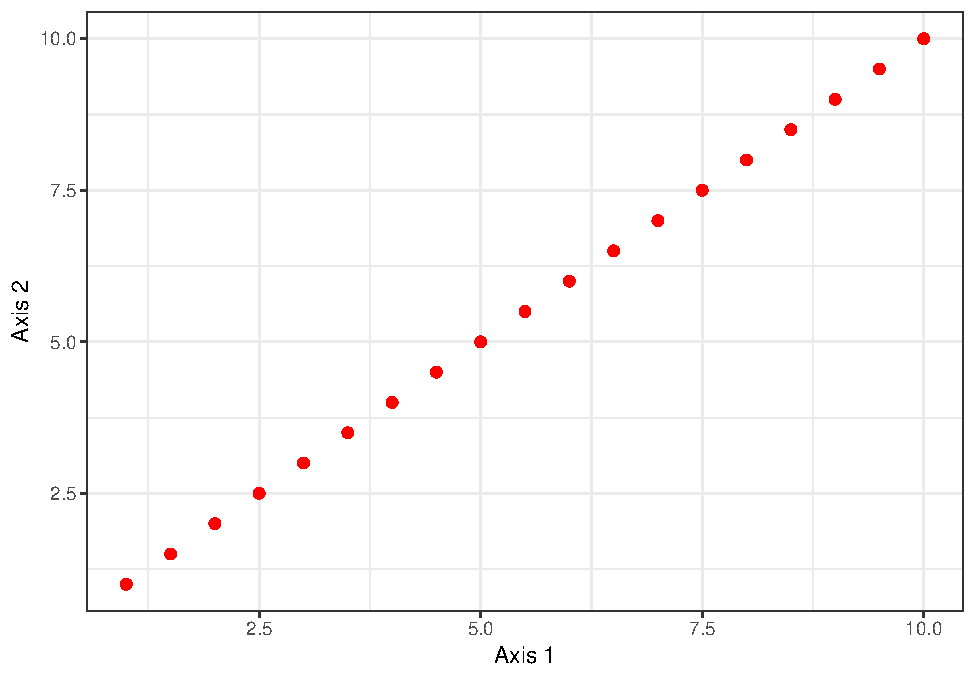
\includegraphics{wickham-thesis_files/figure-latex/fig1-1.pdf}
\caption{A descriptive title about the frequency. \label{fig1}}
\end{figure}

\subsection{Summarize result 2 in a single
sentence.}\label{summarize-result-2-in-a-single-sentence.}

Some great text about this!

\section{Conclusions}\label{conclusions}
\newpage
\singlespacing 
\renewcommand\refname{References}
\bibliography{C:/Users/Victoria/GitHub/wickham-thesis/doc-setup/wickham-thesis-bib}
\end{document}